\documentclass{article}

% preamble
\usepackage{tabularx}
\usepackage{booktabs}
\usepackage{xcolor}
\usepackage{colortbl}
\usepackage{array}
\usepackage{longtable}
\usepackage{graphicx}
\usepackage{url}
\usepackage[left=0.25in, right=0.25in, top=0.5in, bottom=0.5in]{geometry}

% hyperlinks
% filepath: /home/cantabile/Documents/repos/giveadam/observability/obs.tex
\usepackage{hyperref}
\definecolor{darkolive}{RGB}{85, 107, 47}
\hypersetup{
    colorlinks=true,
    linkcolor=darkolive,
    urlcolor=darkolive,
    citecolor=darkolive
}

% title
\title{Questionable analytical observations\\and what to do about them}
\author{Charles T. Gray}

\begin{document}

\maketitle



\begin{abstract}

A critical challenge in data management is balancing complex data transformation with the need for analytic transparency for domain-knowledge validation. FAIR (findable, accessible, interoperable, reusable) data principles as \textit{compliance} fall short when viewed as a checkbox exercise at publication. Living analyses evolve over time, and all analyses are iterative, requiring ongoing validation of data processing decisions. Contemporary data practices on the modern data stack provide robust tooling to validate data transformation, but in practice render data observability opaque to non-technical stakeholders. This creates a fundamental tension between engineering efficiency and analytic interpretability that undermines the core principles of FAIR data.

This document presents a novel tool-agnostic semantic layering methodology for analytic data pipeline design, demonstrated through analysis of UN Sustainable Development Goal (SDG) priorities from dam-affected communities in North India.

The central methodological contribution is a semantically-structured approach to data transformation that extends dbt's engineering-focused patterns to prioritize research interpretability and stakeholder communication. Unlike standard dbt implementations that emphasize technical efficiency, this semantic layering methodology explicitly preserves research context, makes harmonization decisions transparent, and maintains conceptual clarity throughout the data pipeline.

The semantic layer architecture consists of four conceptually distinct stages: source base (raw data cleaning), source entities (region-specific preservation), semantic models (cross-source harmonization), and analytic models (research-ready datasets). This approach addresses the critical gap between technical data engineering practices and research methodology requirements, enabling automated observability while maintaining scholarly rigor.

This semantic layering methodology offers a replicable framework for research data management that bridges the divide between engineering efficiency and research transparency, with applications across all domains requiring multi-source data integration and stakeholder communication.

\end{abstract}

\tableofcontents
\listoftables
\listoffigures


\section{Questionable analytical observations}

Underestimating the complexity of data transformation is a well-recognised driver of garbage in, garbage out data analysis. For example, gene name errors caused by Excel formatting issues are widespread---detected in 700 scientific publications (approximately 20 per cent of 3,500 publications analysed) \cite{ziemann2016gene}. More recently, the UK government's COVID-19 tracking lost about 16,000 cases due to Excel row limits \cite{bbc2020excel}. These examples illustrate how technical limitations and data handling errors can lead to significant analytical inaccuracies.

\subsection{Questionable research practices}

Broadly, the purpose of research is to discover something useful about the world. However, in reality there are so many kinks in the pipeline between the research question and the answer, that the usability and usefulness of the answer that is produced by that pipeline is uncertain. Though, research that passes peer review is often seen as authoritative and accurate. The ‘replication crisis’ movement challenged this, finding that only 1/3 – 1/2 of research, when repeated, finds the same results. This low replication rate has been attributed in part to the use of Questionable Research Practices which make research findings appear more impactful and reliable than warranted by the methods used (Gould et al. in prep). Examples of Questionable Research Practices include HARKing (Hypothesising after results are known), p-hacking (which includes everything from choosing to drop outliers after examining the impact on the results, to rounding p-values down to reach a threshold e.g. p<0.05), and cherry picking (conducting multiple analyses but only presenting the ones with the significant/most publishable results) \cite{john2012measuring}. These practices are prevalent across the fields of science \cite{xie2021prevalence} are indicative of a huge problem in the research pipeline. However, the scope of QRP research has been limited to the analysis and write-up parts of the research pipeline. We argue that the focus on problematic research practices needs to include the earlier parts of the pipeline as well. In this paper we describe “Questionable Analytic Observations” which occur between the point of data collection and the point of analysis, with flow on effects through the rest of the research pipeline. Questionable analytical observations arise when data transformation processes are not transparently validatable or interpretable to domain experts, leading to invisible garbage in, garbage out analytics. This is particularly problematic in multi-source data integration contexts, where harmonization decisions can significantly impact analytical outcomes. 

Sharing code, materials and data is one proposed counter to Questionable Research Practices. This is in line with FAIR principles (see below), facilitates true critical analysis of the analysis methods, and should allow someone to test the method by using the code and data to reproduce the original results. Currently, we are falling well short when it comes to code and data sharing estimates suggesting that across fields 0.5-27% of articles share code and 2-79% share data \cite{hardwicke2018data, culina2020low, stodden2018empirical, kambouris2024computationally, hamilton2023prevalence}. Further, even if this code and data is provided, there is only around a 30% chance that the same answers can be reproduced by a new analyst\cite{hardwicke2018data, kambouris2024computationally}. Clearly, there is a long way to go before an adequate level of transparency is achieved for the analysis component of the research pathway but at least the spotlight is on this issue. The parts of the pipeline between receiving rough-and-ready raw data and beginning the analysis have received almost no attention. In cases where the whole research pipeline is conducted by a single person, and that person is very diligent about documenting their code, methods and data, sometimes these steps are included. However, in other research contexts the research pipeline is carved up between researchers, and data engineers and curators. These circumstances require a premeditated structure to avoid Questionable Analytic Observations that undermine the usefulness and reliability of their results.  

\subsection{What to do about questionable analytical observations}

To address questionable analytical observations, we propose a methodological bridge (Section~\ref{sec:semantic-methodology}) between modern data engineering practices and analytical validation. This involves:
\begin{itemize}
    \item \textbf{Semantic layering of data transformations} to preserve research context and make harmonization decisions explicit (Section~\ref{subsec:core-innovation});
    \item \textbf{Automated observability frameworks} that generate transparent documentation and validation reports from pipeline artifacts (Section~\ref{subsec:obs-table-gen});
    \item \textbf{Stakeholder-centric communication} using conceptual rather than technical terminology to facilitate domain expert validation (Figures~\ref{fig:dbtdag} and \ref{fig:tehri-exclusions});
    \item \textbf{Iterative validation processes} that allow ongoing scrutiny of data processing decisions as analyses evolve over time.
\end{itemize}



\subsection{Case study: giveadam project}

This manuscript and accompanying GitHub repository \href{https://github.com/softloud/giveadam}{\texttt{giveadam}} present a case study implementing the proposed methodology on open science data (Section~\ref{sec:aboutdata}). The project analyzes UN Sustainable Development Goal (SDG) priorities from dam-affected communities in North India, using survey data collected by Garima Gupta from residents of Tehri (where a dam was constructed 20 years ago) and Arunachal Pradesh (where a dam is under development).

This case study demonstrates the methodology on small, analytic data where validation is tractable, but the principles are applicable to large-scale data contexts. To illustrate scalability, the methodology uses open source modern data stack tools standard in enterprise environments, such as Data Build Tool (dbt). The following sections detail the semantic layering methodology, repository architecture, and adherence to FAIR principles.

\section{About the giveadam data}
\label{sec:aboutdata}

The data in this project aggregates two region-based surveys of UN SDG priorities from participants in Tehri and Arunachal Pradesh. Respondents ranked their top three UN SDG priorities, providing insights into development preferences in dam-affected communities. The data is stored in the \texttt{data/} directory of the giveadam repository (see Section~\ref{sec:repository-arch} for complete repository structure). This project aggregates survey responses across regions using the semantic layering methodology (detailed in Section~\ref{sec:semantic-methodology}) to investigate the following research question:

\begin{quote}
  \textit{What are the differences in SDG priorities between residents of Tehri, where a dam was constructed 20 years ago for hydroelectric power, and Arunachal Pradesh, where a dam is currently being developed?}
\end{quote}

Figure \ref{fig:top3-treemap} shows a treemap of the top 3 UN SDG priorities from survey respondents in Tehri (dam constructed 20 years ago) and Arunachal Pradesh (dam under development), North India.

\begin{figure}[ht]
  \centering
  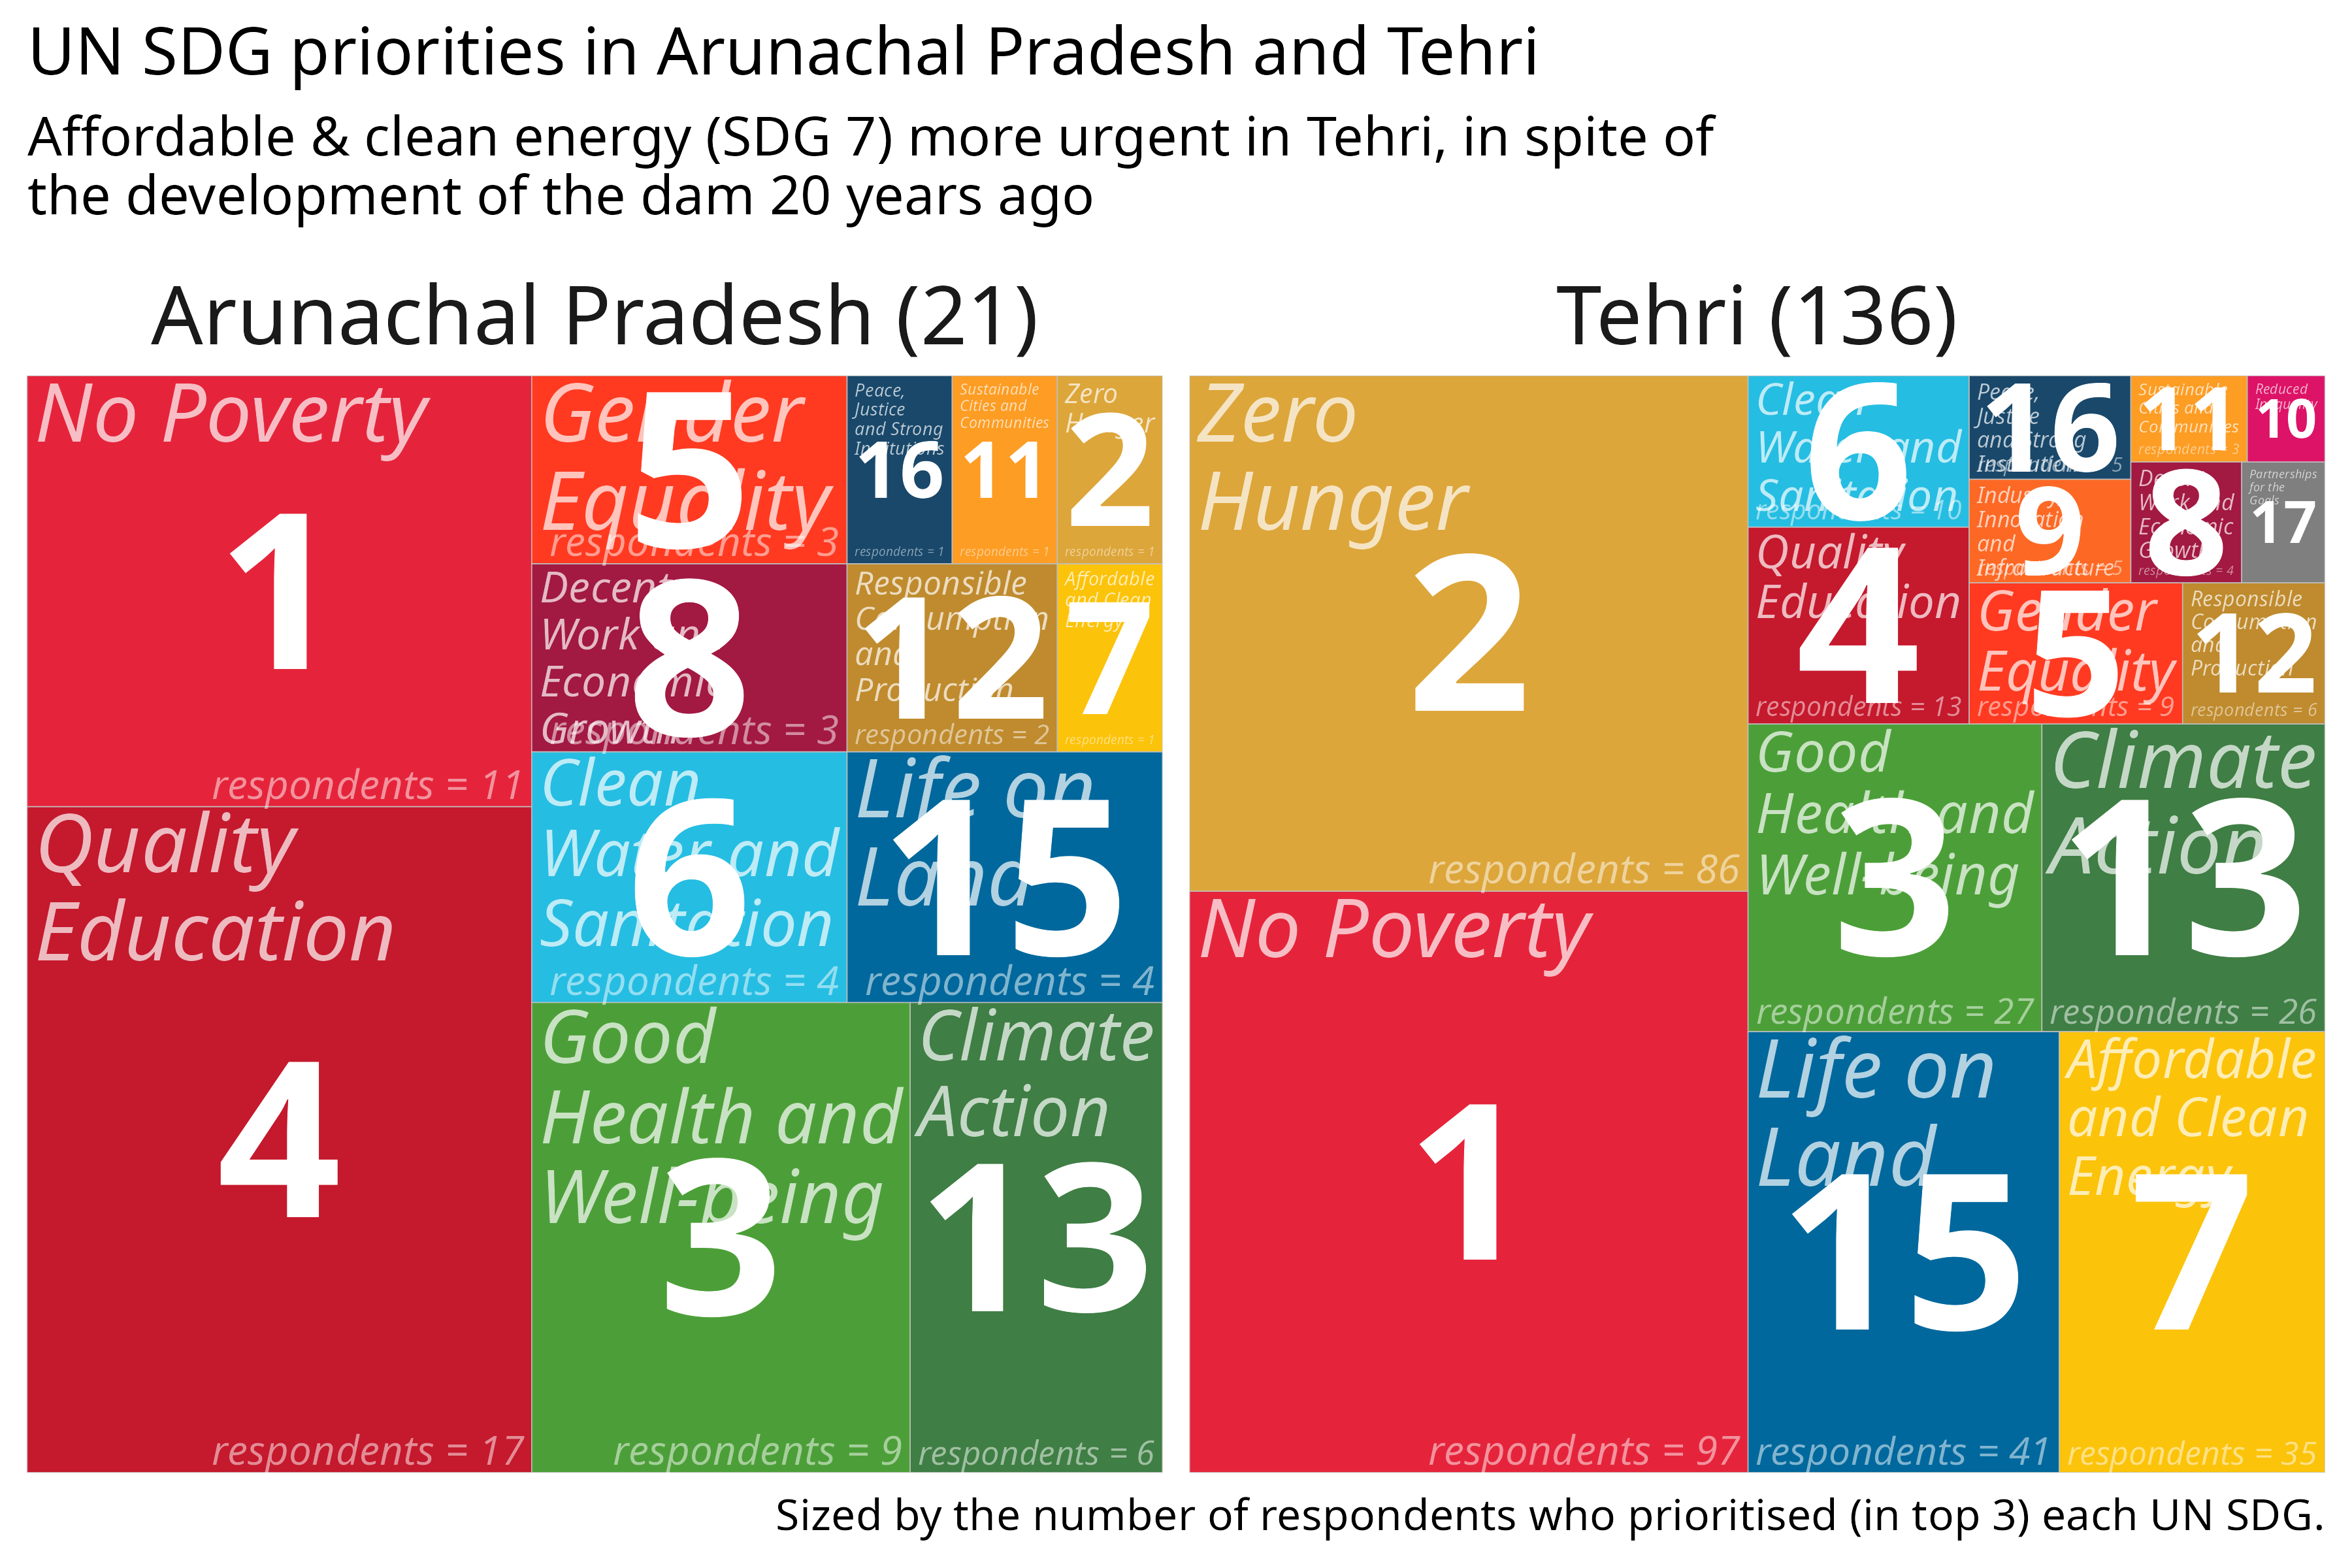
\includegraphics[width=0.95\textwidth]{../figures_and_tables/top3-treemap.png}
  \caption{\label{fig:top3-treemap} Treemap of top 3 UN SDG priorities from survey respondents in Tehri (dam constructed 20 years ago) and Arunachal Pradesh (dam under development), North India. Each rectangle represents a specific UN SDG, with its size proportional to the number of respondents who ranked it among their top three priorities. The treemap visually highlights the most and least prioritized SDGs in each region, providing insights into regional differences in development priorities.}
\end{figure}

By structuring the data in tidy format (one row per ranking by one respondent), the dataset enables flexible analysis across multiple dimensions of respondent characteristics and preferences. 

\section{Semantic data pipeline methodology}
\label{sec:semantic-methodology}

The core methodological innovation of the giveadam project is a semantic layering approach that reconceptualizes data transformation pipelines for research contexts. This methodology addresses a fundamental limitation in current data engineering practices: the tension between technical efficiency and research interpretability within the modern data stack paradigm \cite{modern_data_stack_airbyte}.

\subsection{The semantic layering paradigm}
\label{subsec:semantic-paradigm}

Traditional data engineering prioritizes performance optimization and code maintainability, often at the expense of conceptual clarity for non-technical stakeholders. The semantic layering methodology inverts this priority structure, organizing transformations around research concepts rather than technical convenience. This approach ensures that:

\begin{enumerate}
    \item \textbf{Research context is preserved} throughout the transformation pipeline
    \item \textbf{Harmonization decisions are explicit} and auditable by domain experts  
    \item \textbf{Stakeholder communication} uses conceptual rather than technical terminology
    \item \textbf{Methodological transparency} is maintained without sacrificing automation
\end{enumerate}

\subsection{Repository architecture supporting semantic design}
\label{sec:repository-arch}

The giveadam repository is organized into distinct functional areas:

\begin{itemize}
    \item \textbf{raw\_data/} — Original survey data files as provided by Garima Gupta
    \item \textbf{data/} — Published, analysis-ready datasets (pipeline outputs)
    \item \textbf{dbt\_project/} — Data transformation pipeline with semantic layering
    \item \textbf{observability/} — Automated methodology documentation and quality reports
    \item \textbf{scripts/} — Data preparation and analysis scripts (R, Python)
    \item \textbf{vis-scripts/} — Visualization generation scripts
\end{itemize}

\subsection{Core innovation: Semantic transformation architecture}
\label{subsec:core-innovation}

The central methodological contribution lies in reimagining data transformation layers as conceptual research stages rather than technical processing steps. Standard dbt implementations use staging → intermediate → marts layers optimized for engineering workflows \cite{dbt_docs_structure}. The semantic layering methodology introduces a fundamentally different paradigm:

\begin{itemize}
    \item \textbf{source\_base/} — Raw data integrity and initial cleaning
    \item \textbf{source\_entities/} — Context-preserving regional data entities
    \item \textbf{semantic/} — Explicit cross-source harmonization with documented assumptions
    \item \textbf{analytic/} — Research-question-specific datasets ready for analysis
\end{itemize}

\subsubsection{Why semantic layering transforms research data management}
\label{subsubsec:semantic-benefits}

Each semantic layer addresses specific research methodology requirements:

\begin{enumerate}
    \item \textbf{Context preservation} — Source entities maintain regional survey characteristics, preventing premature harmonization that obscures methodological differences
    \item \textbf{Transparent harmonization} — Semantic models explicitly document how different data sources are reconciled (e.g., SDG labeling differences between regions)
    \item \textbf{Assumption visibility} — Every transformation decision is captured and testable, enabling methodological scrutiny
    \item \textbf{Stakeholder accessibility} — Layer terminology reflects research concepts (semantic, analytic) rather than engineering jargon (staging, marts)
    \item \textbf{Iterative extensibility} — New research questions can be addressed by extending the analytic layer without disrupting upstream logic
\end{enumerate}

This approach resolves the fundamental tension between automated data processing and research transparency, enabling both computational efficiency and methodological rigor.

\subsection{Automated observability for research transparency}

The observability framework generates this methodology documentation automatically from pipeline artifacts, ensuring that:
\begin{itemize}
    \item Documentation remains synchronized with actual transformations
    \item All data quality assumptions are explicitly validated and reported
    \item Research methodology is fully reproducible from code
    \item Stakeholders can verify data processing decisions without technical expertise
\end{itemize}

The complete automated documentation process includes both methodology generation and data publication. The validation tables in this document are generated through the automated process detailed in Section~\ref{subsec:obs-table-gen}. Additionally, \texttt{scripts/publish\_data.R} extracts the final analytic models from the dbt pipeline and exports them as CSV files to the \texttt{data/} directory for publication and external use.

The validation tables presented in this document are high-level summaries. Engineers or researchers requiring deeper pipeline investigation can use \texttt{dbt docs generate} and \texttt{dbt docs serve} for an interactive exploration (e.g., Figure~\ref{fig:tehri-exclusions}) of the complete data lineage (Figure~\ref{fig:dbtdag}), including detailed model specifications, column-level lineage, and test results. 

\begin{figure}[ht]
  \centering
  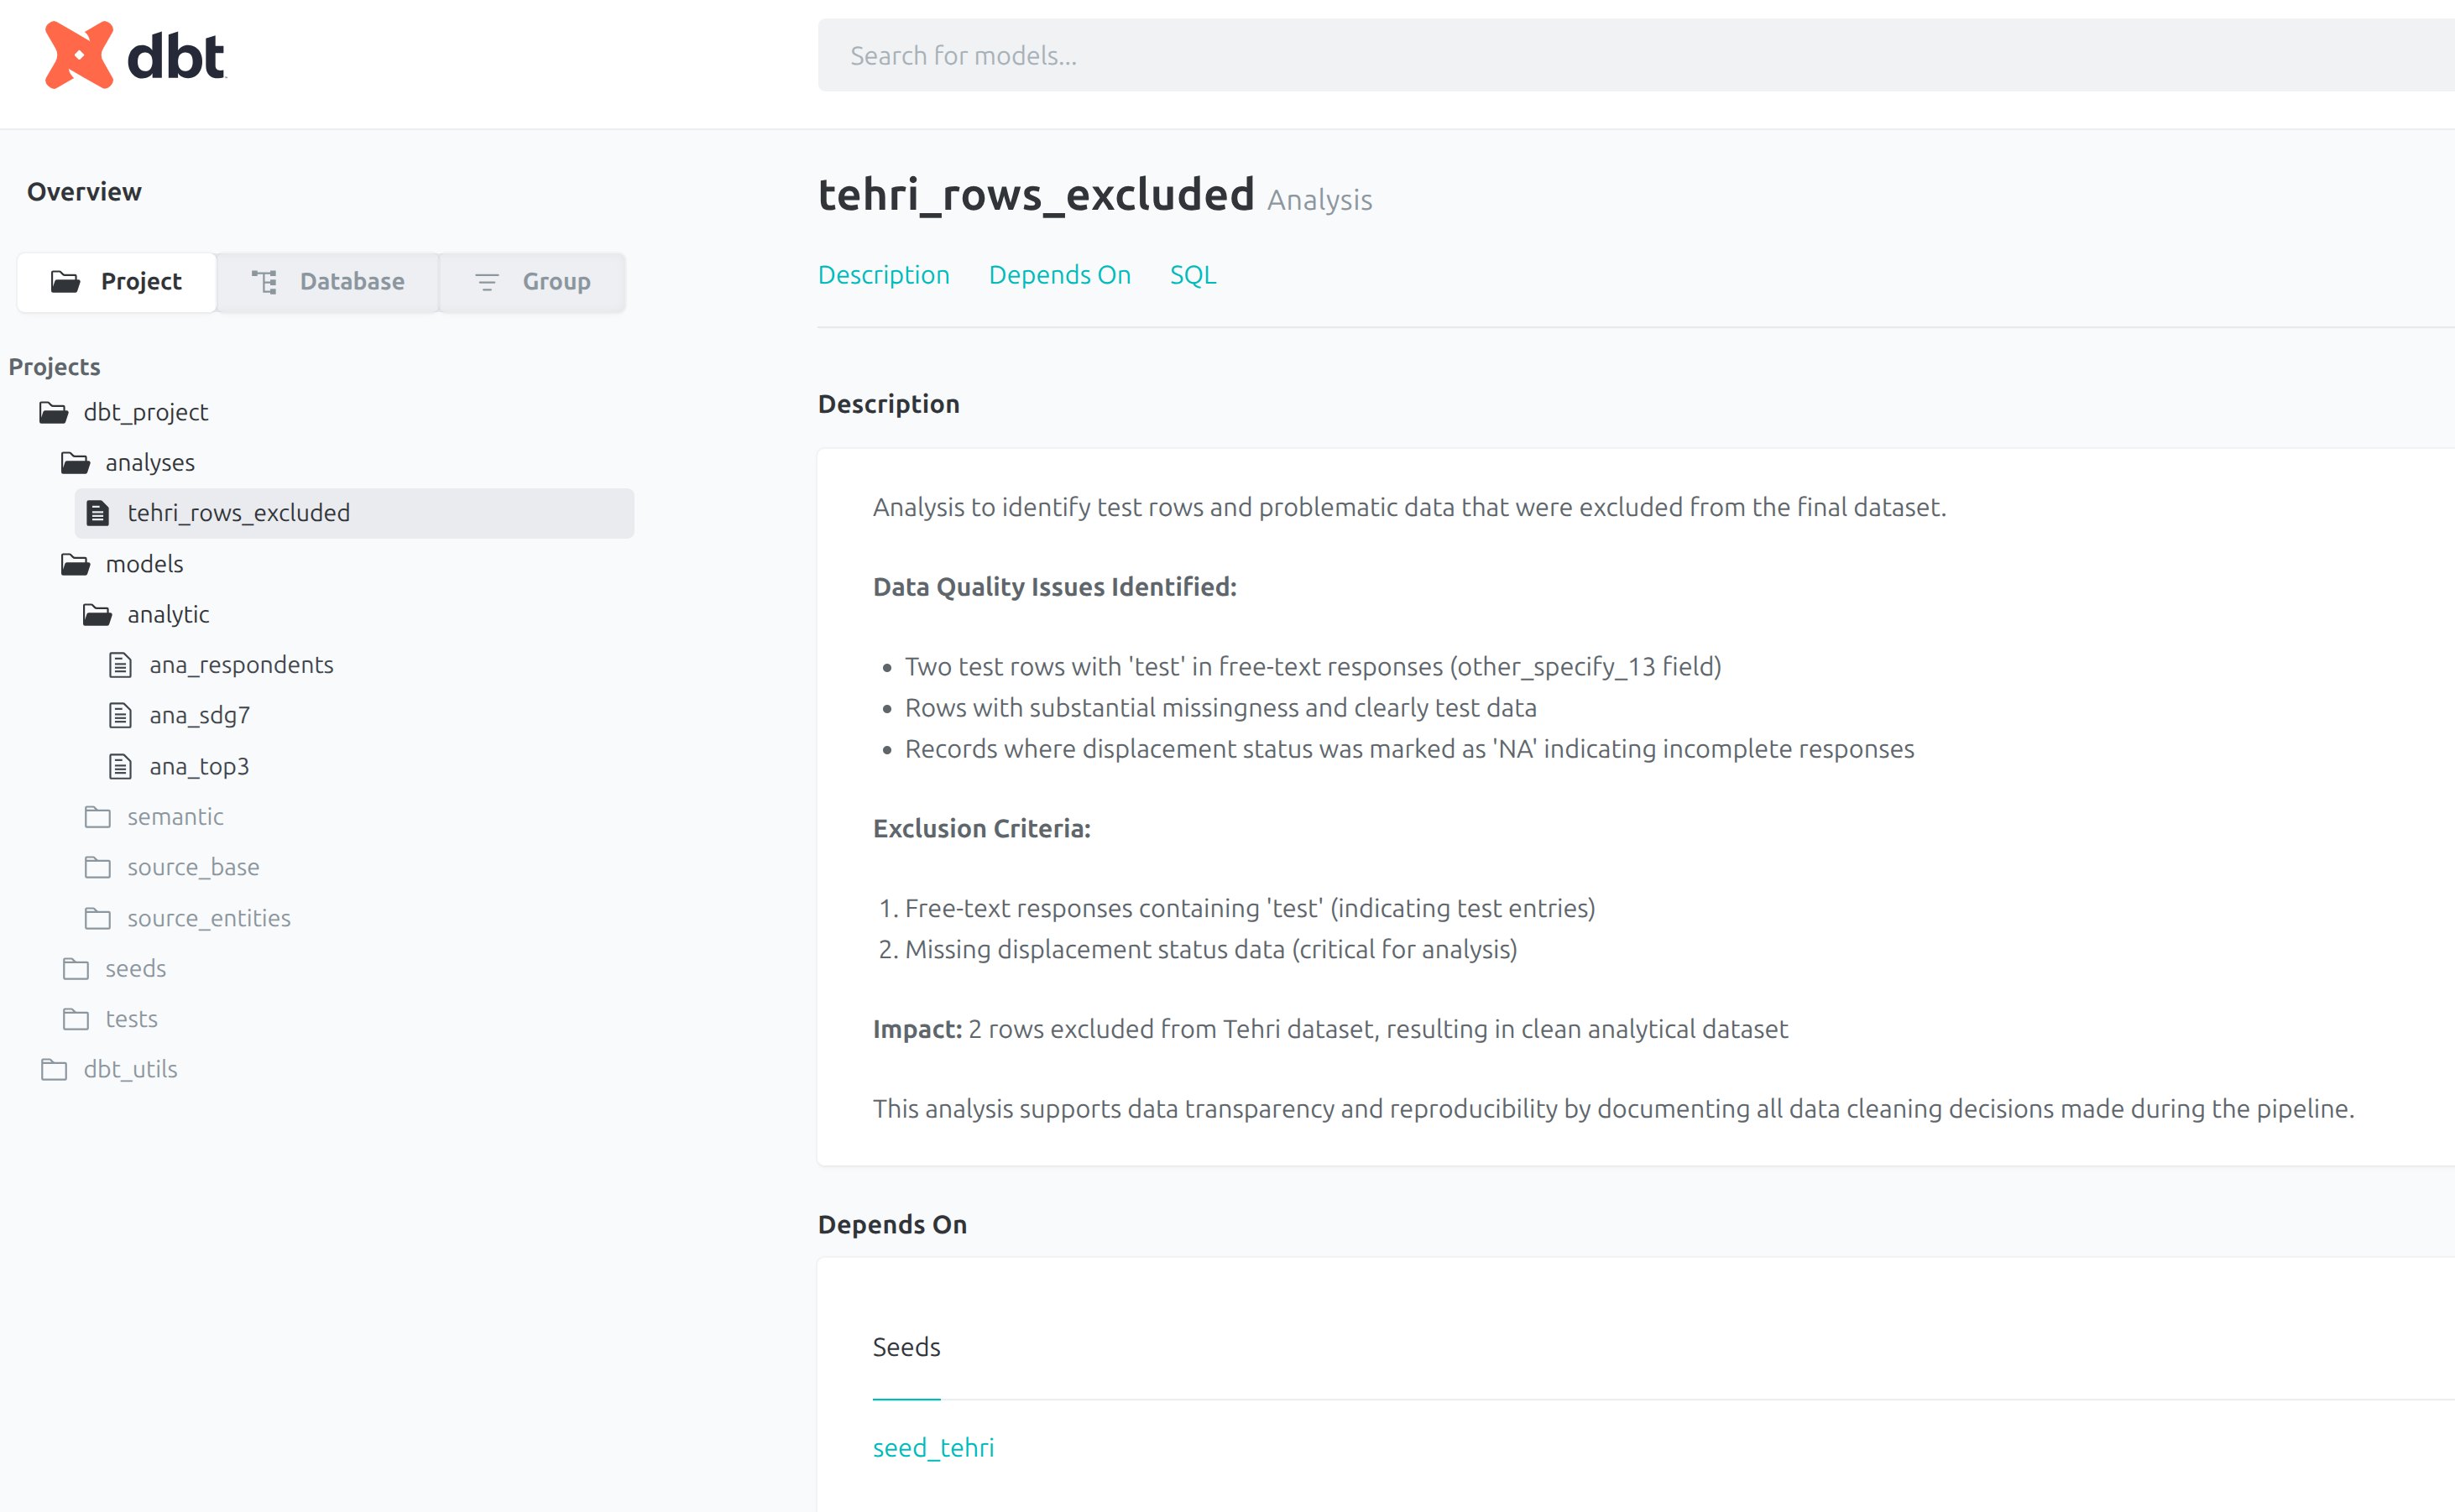
\includegraphics[width=\textwidth]{img/dbt-docs-tehri-exclusions.png}
  \caption{\label{fig:tehri-exclusions} Screenshot from interactive dbt documentation showing the SQL logic excluding two test rows from the Tehri dataset. This exclusion is fully documented in \texttt{dbt\_project/analyses/tehri\_rows\_excluded.sql} and reflects the methodological transparency principles outlined in Section~\ref{sec:semantic-methodology}. DBT documentation provides a user-friendly interface for engineers and stakeholders to verify data processing decisions without requiring technical expertise.}
\end{figure}

\section{FAIR principles implementation}
\label{sec:fair}

The giveadam project implements all four FAIR principles \cite{wilkinson2016fair} through its semantic layering methodology and automated observability framework detailed in Section~\ref{sec:semantic-methodology}. This section demonstrates how the semantic approach enhances traditional FAIR compliance by making research processes themselves findable, accessible, interoperable, and reusable.

\subsection{Findable: Discovery and identification}

\textbf{Rich metadata and identifiers:} The datasets are published with comprehensive metadata in \texttt{data/README.md}, including detailed column descriptions, data provenance, and research context. Each dataset has unique identifiers (\texttt{respondents.csv}, \texttt{SDG\_rankings.csv}) and is version-controlled in the GitHub repository \texttt{giveadam} at \texttt{https://github.com/softloud/giveadam}.

\textbf{Semantic documentation:} Unlike standard data repositories, the semantic layering approach provides findable documentation at multiple conceptual levels. Researchers can locate relevant transformations by research concept (semantic models in Table~\ref{tab:dbt_models}) rather than technical implementation details. The four-layer architecture shown in Figure~\ref{fig:dbtdag} enables discovery through conceptual navigation.

\textbf{Automated cataloging:} The observability framework generates searchable metadata from pipeline artifacts (Table~\ref{tab:dbt_models}), ensuring that all data transformations and quality checks are discoverable through the automated documentation system detailed in Section~\ref{subsec:obs-table-gen}.

\subsection{Accessible: Retrieval and usability}

\textbf{Open access and standard protocols:} Data are published in universally accessible CSV format \cite{csv_rfc} without authentication barriers. The complete repository is openly available via HTTPS and Git protocols \cite{git}, supporting both web browser access and programmatic retrieval through GitHub \cite{github}.

\textbf{Human and machine readable:} Column names follow interpretable conventions prioritizing domain understanding over technical convenience. The semantic layer architecture (Figure~\ref{fig:dbtdag}) ensures that data structure reflects research logic rather than processing efficiency.

\textbf{Multiple access modalities:} Researchers can access data through multiple pathways: direct CSV download, Git repository cloning \cite{git}, or programmatic URL access in R \cite{r_core} or Python \cite{python}. The interactive dbt documentation (\texttt{dbt docs serve}) \cite{dbt_core} provides a web-based interface for exploring complete data lineage.

\subsubsection{SDG rankings dataset}

This dataset contains respondent rankings enriched with demographic metadata:
\begin{itemize}
  \item \textbf{id\_respondent:} Unique identifier for each respondent
  \item \textbf{rank:} Priority ranking (1=highest, 2=medium, 3=lowest priority)
  \item \textbf{sdg\_number:} UN SDG number (1-17)
  \item \textbf{sdg\_label:} Full name of the Sustainable Development Goal
  \item \textbf{age:} Age of respondent in years
  \item \textbf{gender:} Self-reported gender
  \item \textbf{displacement\_status:} Dam impact classification
  \item \textbf{region:} Survey location (tehri, arunachal)
\end{itemize}

By enriching the responses with respondent metadata, we can analyse responses in the context of respondent demographics and characteristics. For example, in Figure~\ref{fig:top3-gender-treemap}, we can see the distribution of top 3 UN SDG priorities by gender.

\begin{figure}[ht]
  \centering
  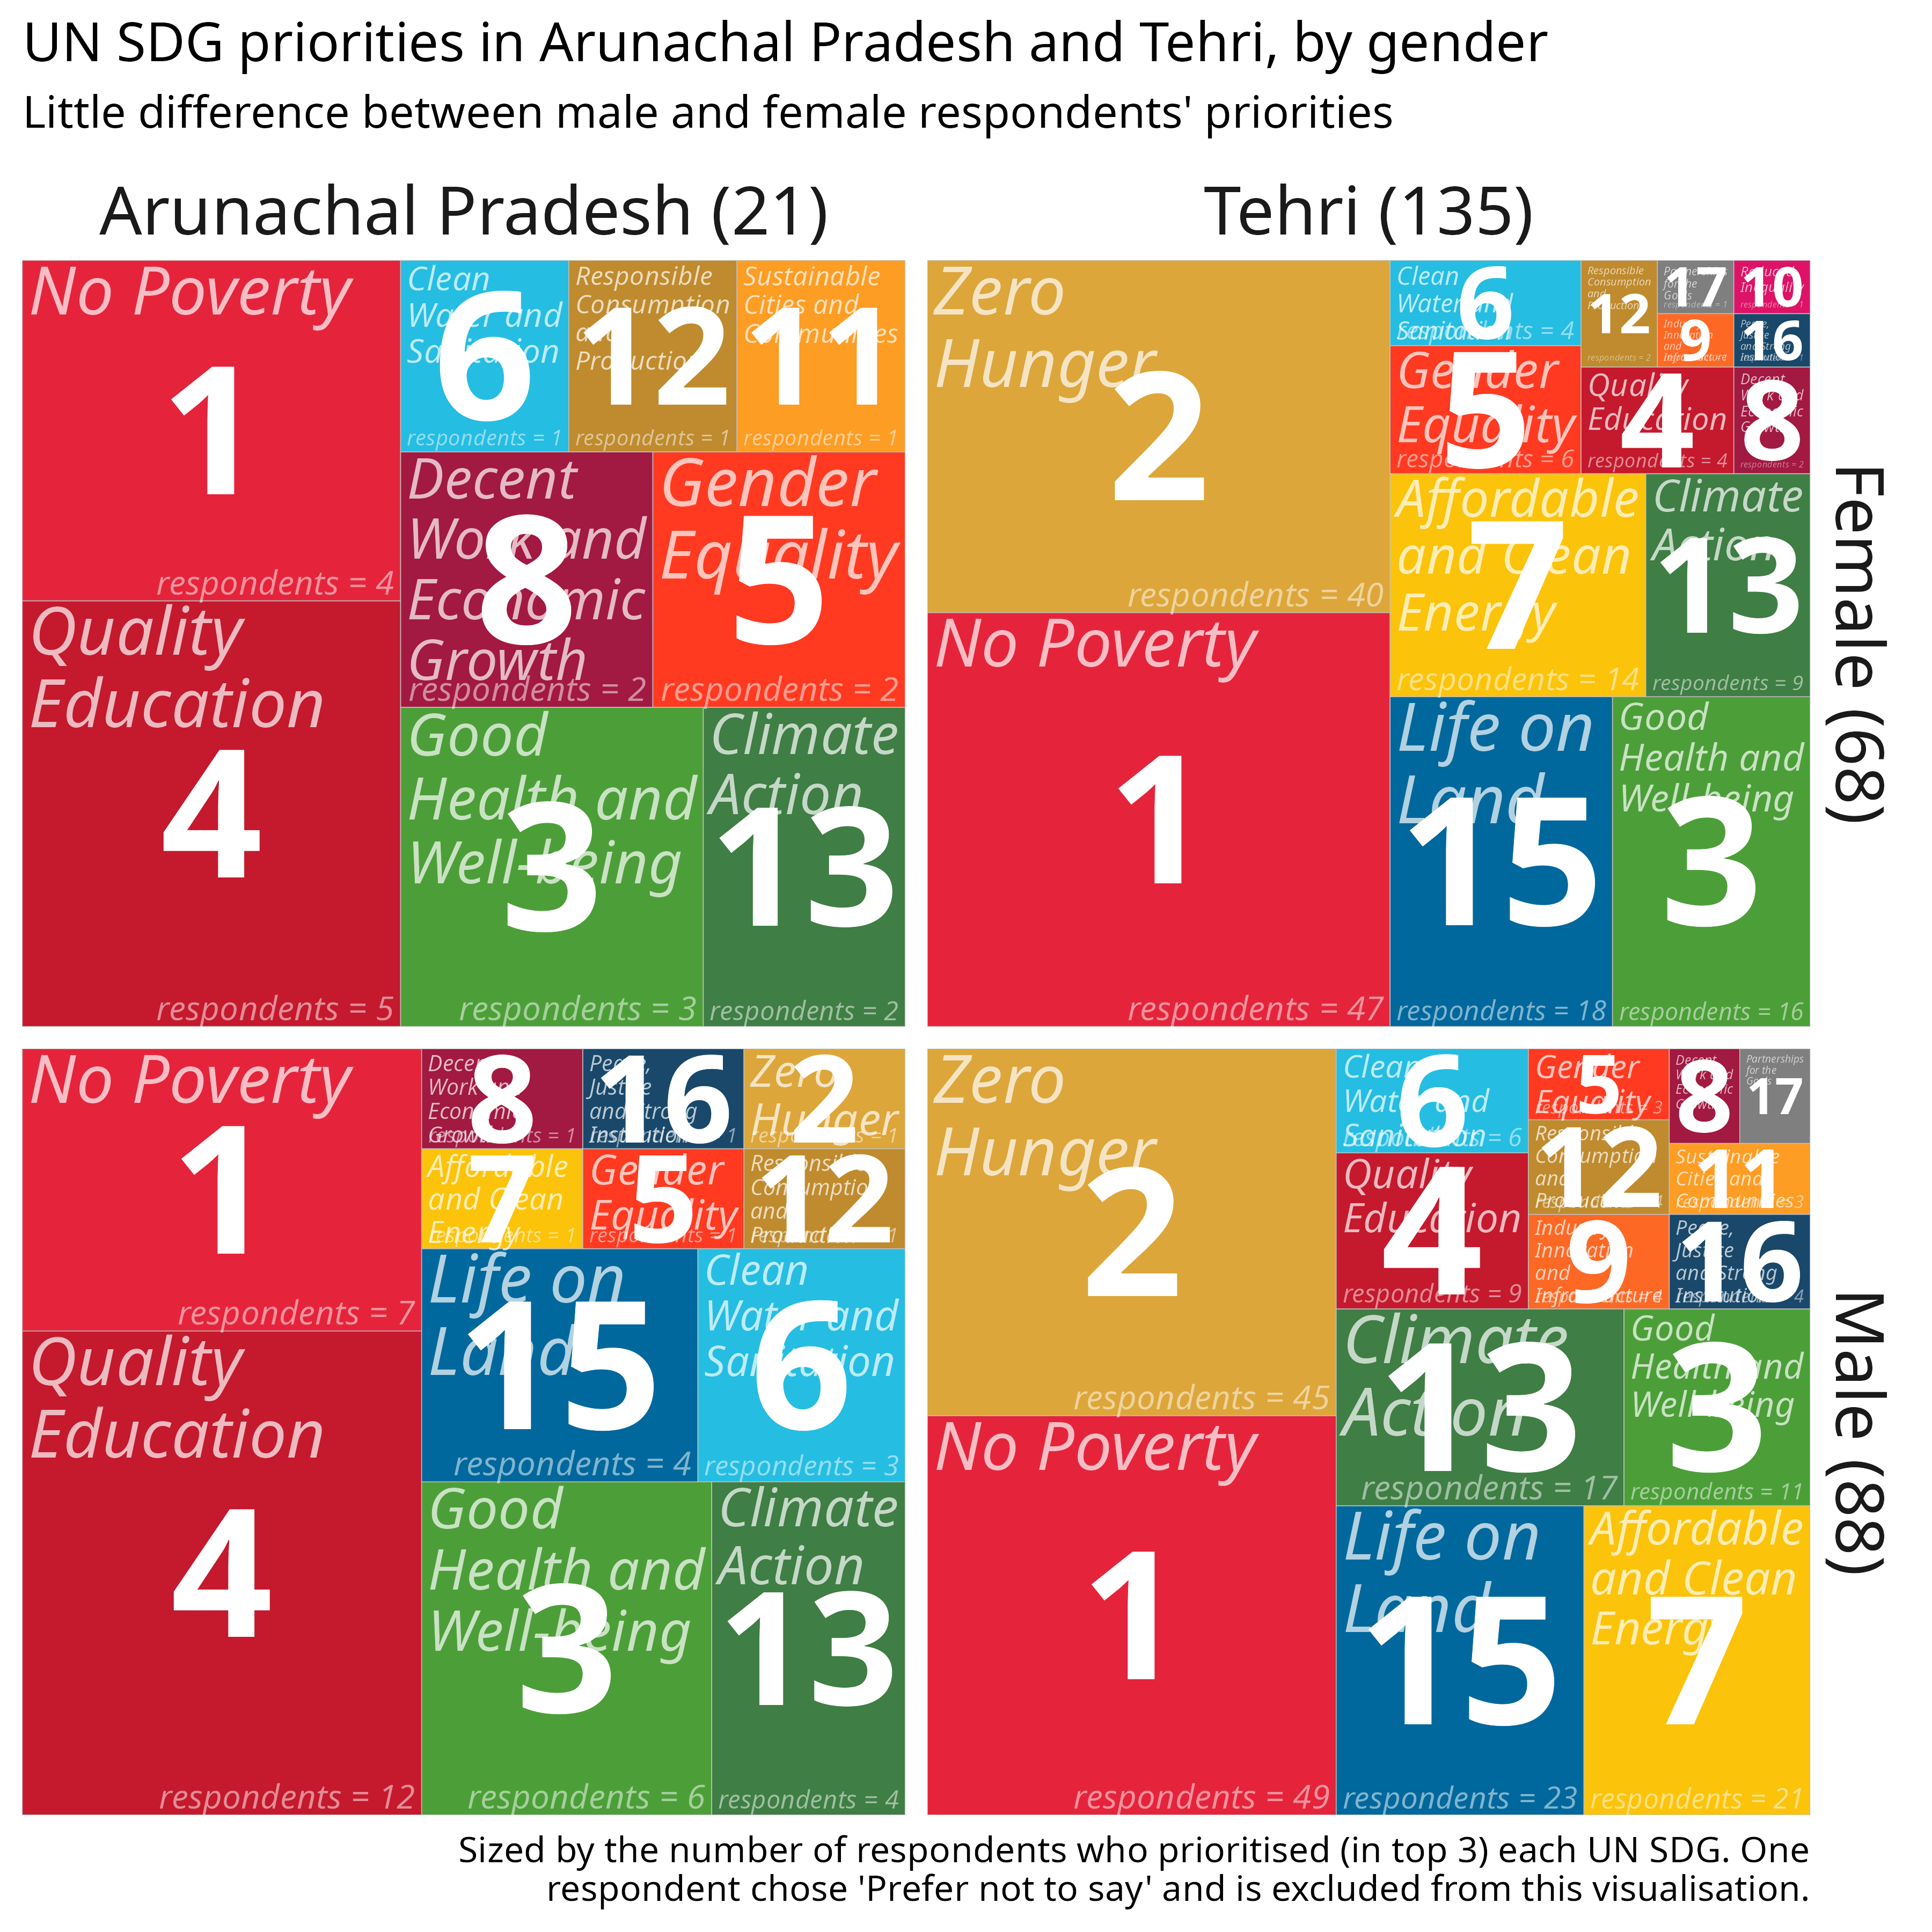
\includegraphics[width=0.95\textwidth]{../figures_and_tables/top3-gender-treemap.png}
  \caption{\label{fig:top3-gender-treemap} Treemap of top 3 UN SDG priorities from survey respondents in Tehri and Arunachal Pradesh, North India, by gender. Each rectangle represents a specific UN SDG, with its size proportional to the number of respondents of a particular gender who ranked it among their top three priorities. The treemap visually highlights the most and least prioritized SDGs in each region, providing insights into gender differences in development priorities.}
\end{figure}

\subsubsection{Respondents dataset}

\begin{itemize}
  \item \textbf{id\_respondent:} Unique identifier for each respondent
  \item \textbf{age:} Age of respondent in years
  \item \textbf{gender:} Self-reported gender (Male, Female, Prefer not to say)
  \item \textbf{displacement\_status:} Impact classification related to dam construction
  \item \textbf{region:} Survey location (tehri, arunachal)
\end{itemize}

\subsection{Interoperable: Integration and exchange}

\textbf{Standard data formats and vocabularies:} Data are published in CSV format \cite{csv_rfc} using UTF-8 encoding with standardized missing value representation (NA). Column naming follows consistent conventions across datasets, enabling seamless joining and integration across the semantic layers shown in Figure~\ref{fig:dbtdag}.

\textbf{Semantic harmonization documentation:} The semantic layer explicitly addresses interoperability challenges by documenting how disparate data sources are harmonized. For example, SDG labeling differences between regional surveys are reconciled with full documentation of mapping decisions in the semantic models (Table~\ref{tab:dbt_models}), enabling other researchers to understand and adapt the harmonization logic.

\textbf{Modular pipeline architecture:} The dbt project structure (Section~\ref{sec:repository-arch}) separates concerns across semantic layers, enabling selective reuse of transformation logic. Researchers can adopt the source entity patterns for context preservation while modifying semantic harmonization for different research domains. Each semantic layer (Table~\ref{tab:dbt_models}) implements specific interoperability functions that can be independently understood and modified.

\textbf{Cross-tool compatibility:} Tidy data principles ensure compatibility across analytical software. The semantic layer structure provides conceptual interoperability—researchers can understand and adapt the methodology regardless of their technical implementation preferences.

\subsection{Reusable: Extension and adaptation}

\textbf{Comprehensive provenance and documentation:} Complete methodology documentation enables confident reuse across research contexts. The automated observability system (Section~\ref{subsec:obs-table-gen}) ensures that documentation evolves with implementation, preventing methodology drift that undermines reusability.

\textbf{Extensible semantic framework:} The semantic layering methodology provides a reusable framework beyond this specific dataset. The four-layer architecture (source base → source entities → semantic → analytic) demonstrated in Figure~\ref{fig:dbtdag} can be adapted for any multi-source research data integration challenge.

\textbf{Quality assurance infrastructure:} The validation framework (Table~\ref{tab:dbt_tests}) provides reusable patterns for data quality verification across research contexts. These automated tests ensure that reused components maintain data integrity standards.

\textbf{Licensing and attribution:} Data are licensed under Creative Commons Attribution 4.0 International (CC BY 4.0) \cite{creative_commons}, enabling broad reuse with appropriate attribution. The license covers both datasets and methodology, encouraging adaptation of the semantic layering approach.

\textbf{Technical infrastructure reusability:} The repository can be forked and the dbt pipeline extended for new data sources or research questions. The modular structure supports iterative development—researchers can extend the analytic layer for new questions without modifying upstream transformations.

\textbf{Methodological transferability:} The semantic layering approach addresses fundamental challenges in research data management that extend beyond this specific domain. The methodology's emphasis on context preservation, transparent harmonization, and stakeholder communication applies to any research requiring multi-source data integration and methodological transparency.

\section{Data lineage}
\label{sec:data-lineage}

\begin{figure}[ht]
\centering
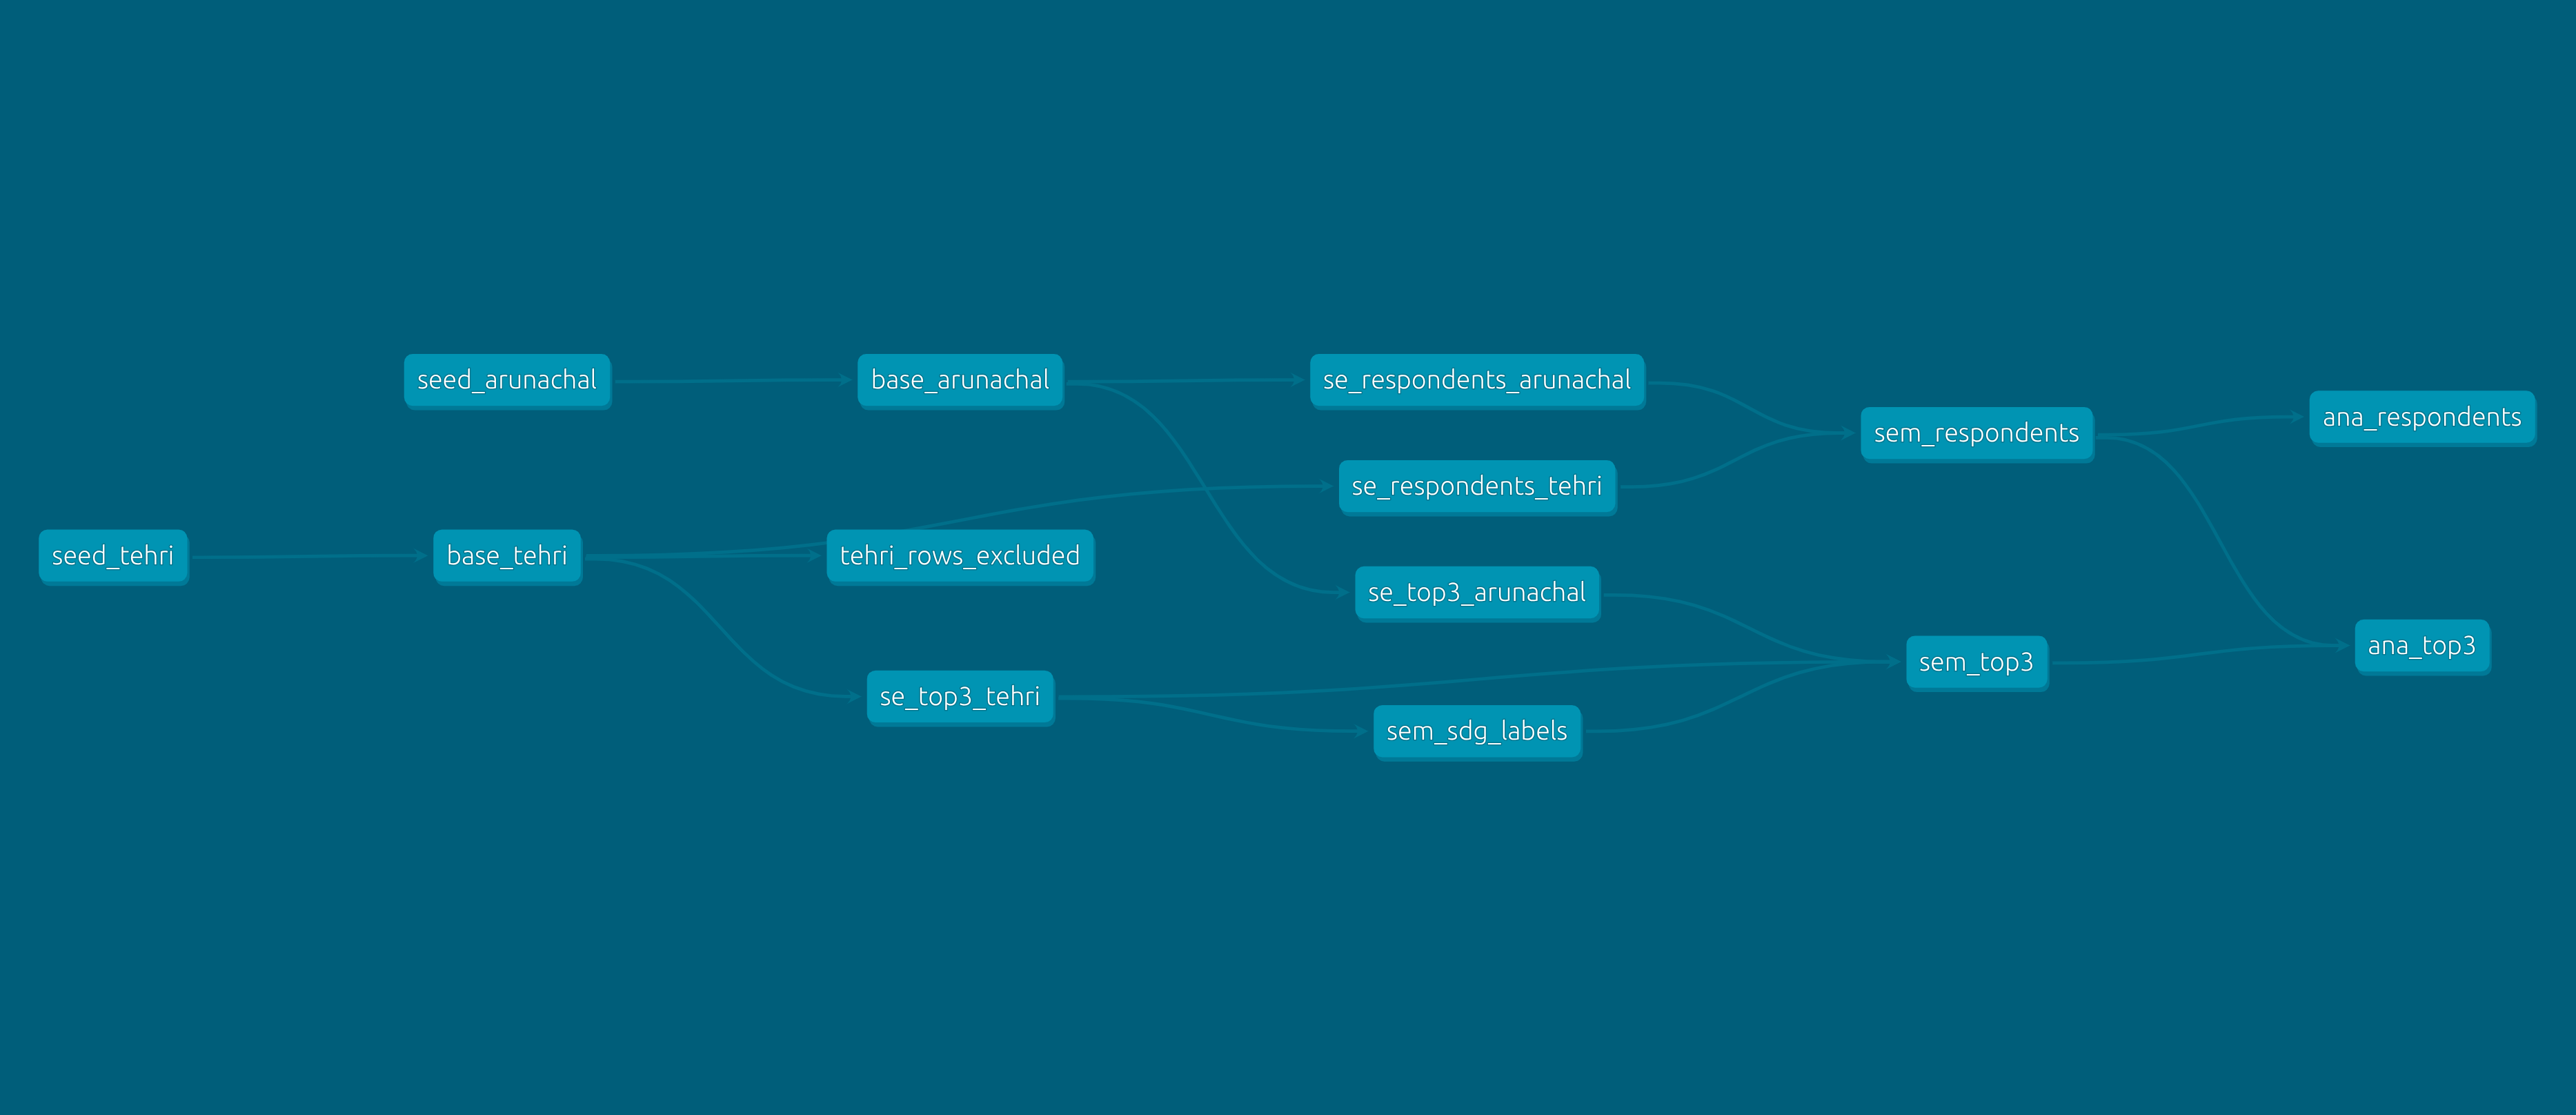
\includegraphics[width=\textwidth]{img/dbt-dag.png}
\caption{Data Build Tool (dbt) directed acyclic graph (DAG) showing the semantic layer structure from source entities through analytic models.}
\label{fig:dbtdag}
\end{figure}

\subsection{Source data and transformation overview}

The giveadam project begins with two regional survey datasets stored in \texttt{raw\_data/}. These datasets required integration across different formats: CSV files \cite{csv_rfc} from Arunachal Pradesh and Excel exports from the Kobo Toolbox \cite{kobo_toolbox} platform for the Tehri region. 

To unify these disparate sources, we implemented a comprehensive data transformation pipeline using the Data Build Tool (dbt) \cite{dbt_core,dbt_duckdb} within the \texttt{dbt\_project/} directory. The complete repository architecture supporting this pipeline is detailed in Section~\ref{sec:repository-arch}.

\subsection{Pipeline architecture and processing}

The transformation pipeline consists of SQL scripts \cite{sql}, automated tests, and comprehensive documentation that convert raw survey data into analysis-ready formats. A significant challenge involved extracting relevant columns from the complex Kobo export structure. We developed a dedicated R script \cite{r_core,tidyverse} (\texttt{scripts/tehri-cols.R}) to identify and map survey questions to data columns, with results documented in \texttt{figure\_and\_tables/tehri\_columns.md} \cite{markdown}.

\subsubsection{Data quality assurance}

Our quality assurance process includes automated identification and exclusion of invalid responses. During processing, we identified and removed two test rows from the Tehri dataset that exhibited substantial missingness and clear indicators of being test data rather than genuine survey responses. This exclusion process is fully documented in \texttt{dbt\_project/analyses/tehri\_rows\_excluded.sql} and reflects the methodological transparency principles outlined in Section~\ref{sec:semantic-methodology}.

\subsection{Visual data flow representation}

Figure~\ref{fig:dbtdag} presents the directed acyclic graph (DAG) generated by dbt for the complete transformation pipeline. This visualization serves multiple purposes:

\begin{itemize}
    \item \textbf{Dependency mapping:} Each node represents a data model or transformation step, while edges show the flow of dependencies between them
    \item \textbf{Layer visualization:} The graph clearly demonstrates the four-layer semantic architecture described in Section~\ref{subsec:semantic-layers}
    \item \textbf{Quality assurance:} The DAG shows how data validation and testing are integrated throughout the transformation process
    \item \textbf{Reproducibility:} The complete lineage enables full reproduction of any analytic dataset from source data
\end{itemize}

This architectural approach ensures data integrity and methodological transparency while enabling efficient processing and clear stakeholder communication.

\subsection{Model catalog and validation}

Table~\ref{tab:dbt_models} provides a comprehensive catalog of all dbt models created within the \texttt{dbt\_project/}, organized by semantic layer. These models implement the semantic extension of dbt's standard layering approach detailed in Section~\ref{subsec:core-innovation}. Each model serves a specific role in the semantic transformation process, from preserving source context to enabling research-ready analysis.

The validation framework supporting these models is documented in Table~\ref{tab:dbt_tests}, which details the automated quality checks applied at each transformation stage. This combination of systematic modeling and rigorous testing ensures both computational efficiency and methodological rigor.

\begin{table}[!h]
\centering
\caption{\label{tab:dbt_models}Data Build Tool (DBT) models created by dbt\_project, ordered by observability layer.}
\centering
\fontsize{8}{10}\selectfont
\begin{tabular}[t]{>{\raggedright\arraybackslash}p{0.18\textwidth}>{\raggedright\arraybackslash}p{0.75\textwidth}}
\toprule
Model & Description\\
\midrule
\addlinespace[0.3em]
\multicolumn{2}{l}{\textbf{Analytic Models}}\\
\hspace{1em}\cellcolor{gray!10}{ana\_respondents} & \cellcolor{gray!10}{Cleaned and transformed respondents data for analysis.}\\
\hspace{1em}ana\_sdg & UN SDG labels and numbers as identifiers.\\
\hspace{1em}\cellcolor{gray!10}{ana\_sdg7} & \cellcolor{gray!10}{Dataset reporting if SDG 7 was prioritised in top 3 ranking by respondents, with respondent metadata.}\\
\hspace{1em}ana\_top3 & Top 3 analytical model for key metrics\\
\addlinespace[0.3em]
\multicolumn{2}{l}{\textbf{Semantic Models}}\\
\hspace{1em}\cellcolor{gray!10}{sem\_respondents} & \cellcolor{gray!10}{Each row represents one respondent in either the survey undertaken in Tehri or the survey undertaken in Arunachale Pradesh.}\\
\hspace{1em}sem\_sdg\_labels & This is a transformation table to integrate SDG labelling across the two survey datasets.\\
\hspace{1em}\cellcolor{gray!10}{sem\_top3} & \cellcolor{gray!10}{Each row a ranking of top 3 SDG priorities, by one respondent from either the Tehri or Arunachal survey. In particular this step ensures that the SDG labels are harmonised across the two surveys.}\\
\hspace{1em}sem\_top3\_arunachal\_long & Long format of top 3 SDG rankings from Arunachal Pradesh respondents.\\
\hspace{1em}\cellcolor{gray!10}{sem\_top3\_tehri\_long} & \cellcolor{gray!10}{Each row represents a respondent's ranking of their top 3 UN Sustainable Development Goals (SDGs) for Tehri, India.}\\
\addlinespace[0.3em]
\multicolumn{2}{l}{\textbf{Source Entity Models}}\\
\hspace{1em}se\_respondents\_arunachal & Each row represents a respondent from Arunachal Pradesh.\\
\hspace{1em}\cellcolor{gray!10}{se\_respondents\_tehri} & \cellcolor{gray!10}{Each row represents a respondent from Tehri.}\\
\hspace{1em}se\_top3\_arunachal & Each row represents a respondent's ranking top 3 UN Sustainable Development Goals (SDGs) for Arunachal Pradesh, India. These data are extracted in wide format from the original survey data preserving labelling for data validation.\\
\hspace{1em}\cellcolor{gray!10}{se\_top3\_tehri} & \cellcolor{gray!10}{Each row represents a respondent's ranking of their top 3 UN Sustainable Development Goals (SDGs) for Tehri, India. These data are extracted in wide format from the original survey data preserving labelling for data validation.}\\
\addlinespace[0.3em]
\multicolumn{2}{l}{\textbf{Base Models}}\\
\hspace{1em}base\_arunachal & Raw data from survey in Arunachal Pradesh, collected by Dr Garima Gupta. Each row represents the survey responses of a single respondent. This step loads the data into the pipeline and establishes an identifier for each respondent. Only top 5 ranking and age and gender in these data, an extraction from the full arunachal dataset which is not available due to institutional restrictions. For this pipeline the top 3 rankings are extracted for analysis.\\
\hspace{1em}\cellcolor{gray!10}{base\_tehri} & \cellcolor{gray!10}{Raw data from survey in Tehri, collected by Dr Garima Gupta. Each row represents the survey responses of a single respondent. This step loads the data into the pipeline and establishes an identifier for each respondent. See `raw\_data/tehri\_cols.md` for details on all questions included in this dataset.}\\
\bottomrule
\end{tabular}
\end{table}


\section{Semantic layer implementation and observability}
\label{sec:semantic-implementation}

The observability framework operationalizes the semantic layering methodology through automated monitoring and validation at each conceptual stage. This implementation demonstrates how semantic design principles translate into technical infrastructure while maintaining research transparency.

\subsection{Semantic layers as methodological framework}
\label{subsec:semantic-layers}

The four-layer semantic architecture serves as both a conceptual framework and technical implementation. Each layer embodies specific research methodology principles:

\begin{itemize}
    \item \textbf{Source Base Models:} Embody the principle of data integrity preservation. These foundational models maintain fidelity to original data sources while implementing only essential cleaning operations. By materializing as seeds, they create an immutable record of processed raw data, enabling complete methodological auditing.

    \item \textbf{Source Entities:} Operationalize the context preservation principle. Each regional dataset maintains its original structure and labeling conventions, preventing premature harmonization. This layer enables validation of regional data characteristics and supports comparative analysis of data collection methodologies.
    
    \item \textbf{Semantic Models:} Implement the transparent harmonization principle. This layer explicitly documents how cross-source differences are resolved, such as reconciling disparate SDG labeling systems. All harmonization logic is encoded in SQL with accompanying documentation, making methodological decisions auditable and modifiable.
    
    \item \textbf{Analytic Models:} Realize the research-readiness principle. These models combine harmonized data with enriched metadata to directly support specific research questions. By materializing as tables, they optimize performance for iterative analysis while maintaining full lineage to upstream decisions.
\end{itemize}

\subsubsection{Methodological advantages of semantic layering}

This semantic architecture delivers specific methodological benefits that standard data engineering approaches cannot provide:

\begin{enumerate}
    \item \textbf{Assumption explicitness:} Every harmonization decision is documented and testable
    \item \textbf{Context preservation:} Regional and methodological differences are maintained until explicitly resolved
    \item \textbf{Stakeholder communication:} Layer names and logic reflect research concepts rather than technical implementation
    \item \textbf{Methodological auditability:} Complete transformation lineage enables scholarly review and replication
    \item \textbf{Iterative extensibility:} New research directions can be accommodated without fundamental restructuring
\end{enumerate}

\subsection{Interactive data exploration}

The validation tables presented in this document provide high-level summaries of data quality and pipeline structure. For comprehensive pipeline investigation, stakeholders can access the full interactive documentation using:

\begin{verbatim}
cd dbt_project/
dbt docs generate
dbt docs serve
\end{verbatim}

This provides an interactive web interface showing detailed model specifications, column-level lineage, test results, and complete data flow visualization.

\subsection{Observability table generation}
\label{subsec:obs-table-gen}

The validation tables presented in this document (Tables~\ref{tab:dbt_models} and~\ref{tab:dbt_tests}) are automatically generated from dbt artifacts to ensure methodology documentation remains synchronized with the actual pipeline implementation.

\subsubsection{Automated metadata extraction}

The observability tables are generated through the following automated process:

\begin{enumerate}
    \item \textbf{dbt artifacts generation} — Running \texttt{dbt build} produces \texttt{manifest.json} and \texttt{run\_results.json} containing complete pipeline metadata
    \item \textbf{Python extraction} — \texttt{create-obs-tables/get-obs-dat.py} extracts model descriptions and test results from JSON artifacts
    \item \textbf{R formatting} — \texttt{create-obs-tables/obs-table.R} formats extracted data into LaTeX tables
    \item \textbf{Document compilation} — LaTeX tables are included in this methodology document via \texttt{\textbackslash input} commands
\end{enumerate}

This automation ensures that any changes to model descriptions, test specifications, or pipeline structure are immediately reflected in the methodology documentation, maintaining complete transparency between implementation and documentation.

\subsubsection{Model materializations}

The semantic layers employ different dbt materializations optimized for their function:

\begin{itemize}
    \item \textbf{Source base models} — Materialized as \texttt{seeds} (CSV files loaded directly into DuckDB)
    \item \textbf{Source entity models} — Materialized as \texttt{views} to preserve disk space while maintaining fast access for downstream models
    \item \textbf{Semantic models} — Materialized as \texttt{views} to enable flexible harmonization logic without storage overhead
    \item \textbf{Analytic models} — Materialized as \texttt{tables} to optimize query performance for research analysis and data export
\end{itemize}

The progression from views to tables reflects the increasing stability and query frequency of models as they approach the analytical layer. Source and semantic layers prioritize flexibility and maintainability through views, while analytic models prioritize performance through table materialization for repeated research queries.

\subsection{Data validation}

Table~\ref{tab:dbt_tests} lists the dbt tests applied to \texttt{dbt\_project/} transformations, ordered by semantic layer. These tests document the data quality assumptions validated at each transformation step in the lineage (Figure~\ref{fig:dbtdag}). The tests ensure data integrity across the semantic pipeline and provide automated quality assurance for research reproducibility.

\begin{table}[!h]
\centering
\caption{\label{tab:dbt_tests}Data Build Tool (DBT) tests applied to dbt\_project models, ordered by observability layer.}
\centering
\fontsize{8}{10}\selectfont
\begin{tabular}[t]{>{\raggedright\arraybackslash}p{0.20\textwidth}>{\raggedright\arraybackslash}p{0.20\textwidth}>{\raggedright\arraybackslash}p{0.10\textwidth}>{\raggedright\arraybackslash}p{0.25\textwidth}>{\raggedright\arraybackslash}p{0.10\textwidth}}
\toprule
Model & Test & Columns & Arguments & Result\\
\midrule
\addlinespace[0.3em]
\multicolumn{5}{l}{\textbf{Analytic Model Tests}}\\
\hspace{1em}\hspace{1em}\cellcolor{gray!10}{ana\_respondents} & \cellcolor{gray!10}{unique\_combination\_of\_columns} & \cellcolor{gray!10}{id\_respondent} & \cellcolor{gray!10}{NA} & \cellcolor{gray!10}{pass}\\
\addlinespace[0.3em]
\multicolumn{5}{l}{\textbf{Semantic Model Tests}}\\
\addlinespace[0.3em]
\multicolumn{5}{l}{\textbf{Source Entity Tests}}\\
\hspace{1em}\hspace{1em}se\_respondents\_arunachal & accepted\_values & gender & Male\_\_Female\_\_Prefer\_not\_to\_say & pass\\
\hspace{1em}\cellcolor{gray!10}{se\_respondents\_arunachal} & \cellcolor{gray!10}{not\_null} & \cellcolor{gray!10}{id\_respondent} & \cellcolor{gray!10}{NA} & \cellcolor{gray!10}{pass}\\
\hspace{1em}se\_respondents\_arunachal & unique & id\_respondent & NA & pass\\
\hspace{1em}\cellcolor{gray!10}{se\_respondents\_arunachal} & \cellcolor{gray!10}{unique\_combination\_of\_columns} & \cellcolor{gray!10}{id\_respondent} & \cellcolor{gray!10}{NA} & \cellcolor{gray!10}{pass}\\
\hspace{1em}se\_respondents\_tehri & accepted\_values & gender & Male\_\_Female\_\_Prefer\_not\_to\_say & pass\\
\hspace{1em}\cellcolor{gray!10}{se\_respondents\_tehri} & \cellcolor{gray!10}{not\_null} & \cellcolor{gray!10}{id\_respondent} & \cellcolor{gray!10}{NA} & \cellcolor{gray!10}{pass}\\
\hspace{1em}se\_respondents\_tehri & unique & id\_respondent & NA & pass\\
\hspace{1em}\cellcolor{gray!10}{se\_respondents\_tehri} & \cellcolor{gray!10}{unique\_combination\_of\_columns} & \cellcolor{gray!10}{id\_respondent} & \cellcolor{gray!10}{NA} & \cellcolor{gray!10}{pass}\\
\hspace{1em}se\_top3\_arunachal & accepted\_values & rank & 1\_\_2\_\_3 & pass\\
\hspace{1em}\cellcolor{gray!10}{se\_top3\_arunachal} & \cellcolor{gray!10}{not\_null} & \cellcolor{gray!10}{id\_respondent} & \cellcolor{gray!10}{NA} & \cellcolor{gray!10}{pass}\\
\hspace{1em}se\_top3\_arunachal & unique\_combination\_of\_columns & id\_respondent & rank & pass\\
\hspace{1em}\cellcolor{gray!10}{se\_top3\_tehri} & \cellcolor{gray!10}{accepted\_values} & \cellcolor{gray!10}{rank} & \cellcolor{gray!10}{1\_\_2\_\_3} & \cellcolor{gray!10}{pass}\\
\hspace{1em}se\_top3\_tehri & not\_null & id\_respondent & NA & pass\\
\hspace{1em}\cellcolor{gray!10}{se\_top3\_tehri} & \cellcolor{gray!10}{unique\_combination\_of\_columns} & \cellcolor{gray!10}{id\_respondent} & \cellcolor{gray!10}{rank} & \cellcolor{gray!10}{pass}\\
\addlinespace[0.3em]
\multicolumn{5}{l}{\textbf{Base Model Tests}}\\
\hspace{1em}base\_arunachal & unique\_combination\_of\_columns & id\_respondent & NA & pass\\
\hspace{1em}\cellcolor{gray!10}{base\_arunachal} & \cellcolor{gray!10}{unique\_combination\_of\_columns} & \cellcolor{gray!10}{respondents} & \cellcolor{gray!10}{NA} & \cellcolor{gray!10}{pass}\\
\hspace{1em}base\_tehri & not\_null & id\_respondent & NA & pass\\
\hspace{1em}\cellcolor{gray!10}{base\_tehri} & \cellcolor{gray!10}{unique} & \cellcolor{gray!10}{id\_respondent} & \cellcolor{gray!10}{NA} & \cellcolor{gray!10}{pass}\\
\hspace{1em}base\_tehri & unique\_combination\_of\_columns & id & NA & pass\\
\hspace{1em}\cellcolor{gray!10}{base\_tehri} & \cellcolor{gray!10}{unique\_combination\_of\_columns} & \cellcolor{gray!10}{id\_respondent} & \cellcolor{gray!10}{NA} & \cellcolor{gray!10}{pass}\\
\bottomrule
\end{tabular}
\end{table}


\section{Use of NLP tools}

The giveadam project architecture, semantic data pipeline design, and all data transformations were conceived and implemented by Charles T. Gray. GitHub Copilot \cite{copilot} was used for documentation editing and selected development operations tasks (supporting JSON manifest parsing scripts), but did not contribute to the fundamental design decisions, data modeling approach, or core analytical implementations. All code development, methodological innovations, and research insights represent the original work of the author.

\section{Acknowledgements}

The author gratefully thanks Garima Gupta for collecting and sharing the original survey data from Tehri and Arunachal Pradesh, North India. The author also acknowledges the open-source software community for developing the tools that made this project possible, including dbt, DuckDB, R, Python, and their associated libraries.

\bibliographystyle{plain}
\bibliography{references}

\end{document}
